\documentclass[10pt]{article}

% Default 
\usepackage{graphicx}
\usepackage[
  backend=biber,
  style=numeric, 
  sorting=none
]{biblatex}

% Additional
\usepackage{amsmath}
\usepackage{textcomp, gensymb}
\usepackage{placeins}
\usepackage{tabularray} 
\usepackage{xcolor}
\usepackage{placeins}
\usepackage{csquotes} 
\usepackage{todonotes}
\usepackage{hyperref}
\usepackage{siunitx}

\newcommand{\td}[1]{\todo[linecolor=blue, backgroundcolor=blue!25,bordercolor=blue, size=\small, inline]{#1}}

\addbibresource{references.bib}

\title{Microwave Optics 2} 
\author{Rahmanyaz Annyyev, Hikmat Gulaliyev}
\date{9 May, 2024} 

\begin{document}

\maketitle

\td{I have a class early in the morning so I gotta go to sleep. I can wrap up abstract and some other bullshit after the class.}

\begin{abstract}

\end{abstract}

\section{Introduction}

\subsection*{General}

The Gunn diode transmitter is a non-linear device used in high-frequency electronics. It consists of a $10.525$ GHz Gunn diode, or a transferred electron device (TED)---a two-terminal semiconductor that generates the radiation, a microwave horn antenna that emits the radiation, and a $18$ cm high stand that reduces surface top reflections. The Gunn diode is located within a $10.525$ GHz resonant cavity. The transmitter has a power output of $15$ mW, and emits coherent, linearly polarized microwaves at a wavelength of $28.5$ mm along the axis of the diode through the horn antenna. It is powered from a standard $115$ or $220/240$ VAC, $50/60$ Hz outlet.

The microwave receiver is a non-linear device used to detect the radiation emitted by the transmitter. Its main components are a microwave horn antenna that collects the radiation, a Schottky diode detector that converts the radiation into a DC signal, and a $18$ cm high stand that reduces surface top reflections. The diode detector responds only to the component of the signal that is polarized along the axis of the diode and is located within a $10.525$ GHz resonant cavity. The readings of the receiver are approximately proportional to the intensity of the radiation for low amplitude signals. The receiver has an adjustable intensity knob that can be used to set the sensitivity of the receiver. At each setting, the readings must be multiplied by a constant factor to obtain the actual intensity of the radiation. The receiver has four settings: $1$, $3$, $10$, and $30$. 

In this experiment, we will study the interference of microwaves that pass through a double slit and the division of amplitude of microwaves that are reflected by a partial reflector. The interference of microwaves is a wave phenomenon that occurs when two or more waves overlap in space. 

In the case of a double slit, the microwaves that pass through the slits interfere with each other, creating a pattern of alternating bright and dark fringes on a screen. For two slits separated by a distance $d$, the angle $\theta$ between the central maximum and the first-order maximum is given by the formula $\sin \theta = \lambda/d$, where $\lambda$ is the wavelength of the microwaves. 

In the case of a partial reflector, the microwaves that are reflected by the surface interfere with the microwaves that are transmitted through the surface, creating a pattern of alternating bright and dark fringes on a screen.

\subsection*{Procedure} 

The experiment is comprised of two parts: A and B. The setup consists of a Gunn diode transmitter, a microwave receiver, one narrow and two wide slit spacers, a partial and a metal reflectors, a component holder, a slit extender arm, and rotating goniometer.

\subsubsection*{Part A}

The purpose of the first part of the experiment is to observe the intensity of the microwave radiation as a function of the angle of the transmitter due to interference, specifically the division of the wavefront.

We first construct a double slit using the narrow slit spacer, the slit extender arm, and two reflectors as shown in Figure~\ref{fig:1}. It should be symmetrical and the slits should be parallel to each other with widths of $15$ mm. The transmitter and receiver are placed at the same height on the goniometer. Next, the transmitter and reciever are configured for vertical polarization. The transmitter is then rotated to $0\degree$ and the receiver is adjusted to read $1$. The transmitter is then rotated in $5\degree$ increments in the clockwise direction and the receiver readings are recorded in a table. The same procedure is repeated for the counter-clockwise direction. Occasionally, the differences between readings at consecutive angles might be signigicant. In such cases, the intensity readings at intermediate angles should be analyzed.

\begin{figure}[hbt!]
  \centering
  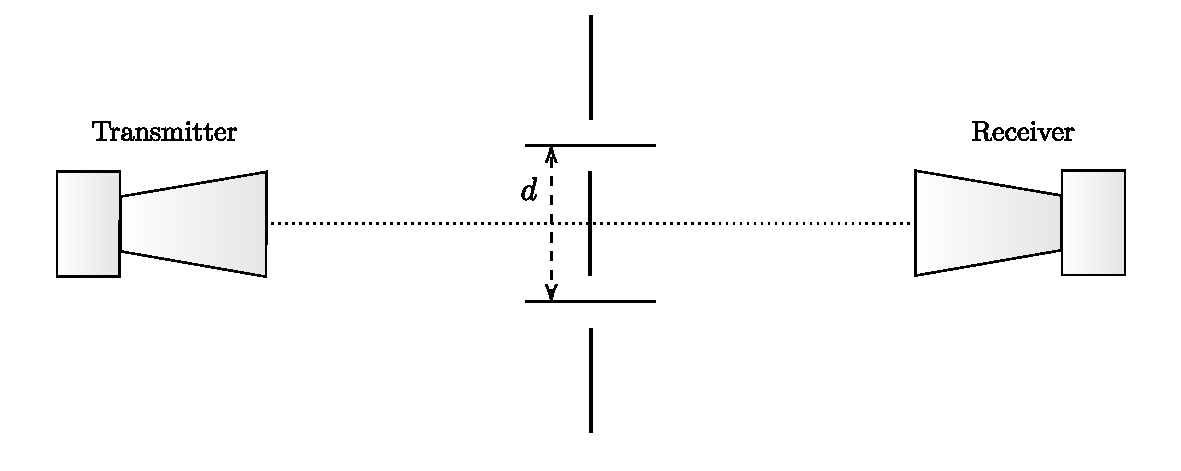
\includegraphics[scale=0.6]{figures/f1.pdf}
  \caption{The setup for the first part of the experiment.}
  \label{fig:1}
\end{figure}

A variation in the setup could be introduced by using a wide slit spacer instead of the narrow one. The former is $90$ mm wide, whereas the latter is $60$ mm wide. To ensure the same relative intensity at the slits in such a case, the receiver should be moved back by $50$%.

\subsubsection*{Part B}

The objective of the second part of the experiment is to examine the intensity of the microwave radiation as a function of the position of the receiver due to interference, particularly the division of amplitude.

We first assemble the setup as shown in Figure~\ref{fig:2}. The transmitter is facing the partial reflector, and the receiver is placed slightly behind the transmitter so that it does not receive a direct signal. A metal reflector is then placed behind the partial reflector, parallel to it. Next, the receiver is slowly moved along the goniometer until the intensity of the signal is minimized or maximized. The position of the receiver at either of these points is recorded. 

\begin{figure}[hbt!]
  \centering
  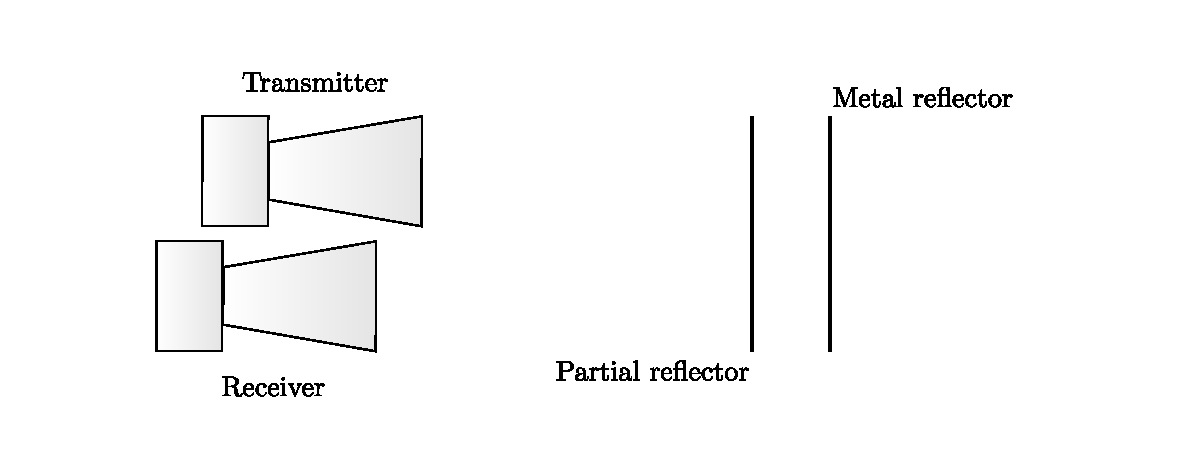
\includegraphics[scale=0.6]{figures/f2.pdf}
  \caption{The setup for the second part of the experiment.}
  \label{fig:2}
\end{figure}

\section{Data \& Results}

\subsection*{Part A}

The data obtained in the first part of the experiment is shown in Table~(\ref{tab:1}).

The plot of the intensity readings as a function of the angle of the transmitter is shown in Figure~(\ref{fig:3}).
According to the theory, maximas should occur at $0\degree$, $28.4\degree$, $71.8\degree$, whereas minimas should occur at $13.7\degree$, $28.4\degree$, $45.4\degree$, and thereafter.
Experimentally, the maximas are observed at $0\degree$, $25\degree$, and minimal at $15\degree$, $45\degree$. The values after 50 degrees are approximately 0, as intensity readings are less than the detection limit.

As per the reason for the drop in intensity between successive maximas, it is due to the division of the wavefront. As we move towards higher order maximas, number of interfering wavefronts drops, leading to a decrease in intensity. 
\begin{figure}
  \centering
  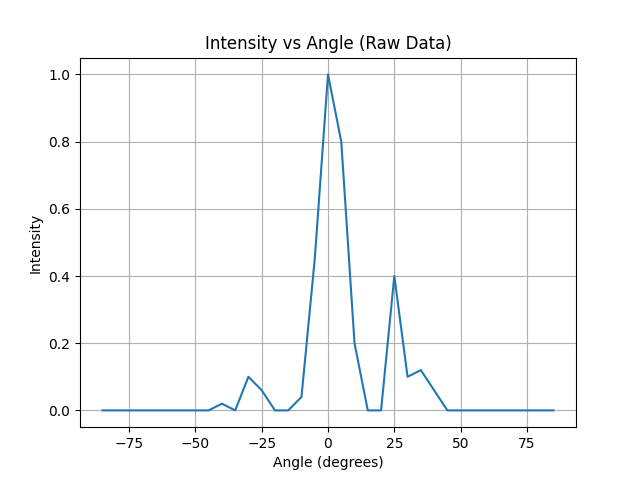
\includegraphics[scale=0.6]{plots/plot1.png}
  \caption{Intensity readings as a function of the angle of the transmitter.}
  \label{fig:3}
\end{figure}
\td{update the plot}
\begin{table}[ht]
  \centering
  \begin{tblr}{
    cells = {halign = c, valign = m},
    row{odd} = {bg = lightgray!5},
    row{1} = {bg = lightgray!20},
    hlines = {},
    vlines = {}
  }
    Angle & {Clockwise \\ Int. Read.} & {Counter. \\ Int. Read.} & Angle & {Clockwise \\ Int. Read.} & {Counter. \\ Int. Read.} \\
    \hline 
    0\degree & 1 & 1 & 45\degree & 0 & 0 \\
    5\degree & 0.45 & 0.8 & 50\degree & 0 & 0 \\
    10\degree & 0.04 & 0.2 & 55\degree & 0 & 0 \\
    15\degree & 0 & 0 & 60\degree & 0 & 0 \\
    20\degree & 0 & 0 & 65\degree & 0 & 0 \\
    25\degree & 0.06 & 0.4 & 70\degree & 0 & 0 \\
    30\degree & 0.1 & 0.1 & 75\degree & 0 & 0 \\
    35\degree & 0 & 0.12 & 80\degree & 0 & 0 \\
    40\degree & 0.02 & 0.06 & 85\degree & 0 & 0 \\
  \end{tblr}
  \caption{Results of the first part of the experiment.}
  \label{tab:1}
\end{table}

\subsection*{Part B}

The data obtained in the second part of the experiment is shown in Table~(\ref{tab:2}).

\begin{table}[ht]
  \centering
  \begin{tblr}{
    cells = {halign = c, valign = m},
    column{1} = {bg = lightgray!20},
    hlines = {},
    vlines = {}
  }
    {Reflector Pos. \\ for Max. (or Min.)} & $71.2$ & $72.7$ & $74.5$ & $76$ & $77.4$ & $79$ \\
  \end{tblr}
  \caption{Results of the second part of the experiment.}
  \label{tab:2}
\end{table}

The average difference between the values is calculated using the formula 
\begin{equation}
  \Delta x = \dfrac{1}{n} \sum_{i=1}^{n-1} |x_i - x_{i+1}|
\end{equation}
where $x_i$ is the intensity reading at the $i$th position of the receiver. It is found to be $13$ mm which is approximately equal to half the wavelength of the microwaves $\lambda/2 = 14.25$ mm.

The reason behind this phenomenon is that consecutive maxima and minima of the intensity of the microwaves are separated by half the wavelength of the microwaves.



\section{Discussion \& Conclusion}

\subsection*{Errors}
There are a few sources of error such as the detection limit of the receiver, the alignment of the transmitter and receiver, stability of the setup, and human error.

\begin{itemize}
  \item \textbf{Detection Limit:} The intensity readings of the receiver are limited by the sensitivity of the receiver. The readings are not accurate for intensities below the detection limit of the receiver. Therefore limiting the amount of data collected. 
  \item \textbf{Alignment:} The alignment of the transmitter and receiver is crucial for accurate readings. Since the alignment is done manually, there is a possibility of human error.
  \item \textbf{Stability:} The stability of the setup is important for accurate readings. Vibrations and other disturbances were affecting the reading of the receiver.
  \item \textbf{Human Error:} There is a possibility of human error in reading the intensity of the microwaves on the receiver.
  \item \textbf{Measurement interval:} The measurements were taken at $5\degree$ intervals. This introduces at least $2.5\degree$ error in the location of each maxima and minima.
\end{itemize}

\subsection*{Approximations}
\begin{itemize}
  \item \textbf{Coherence of the microwaves:} The microwaves are assumed to be homogenous and coherent. In reality, the microwaves are not perfectly homogenous and coherent.
  \item \textbf{Reflections:} Metal reflector is assumed to be perfectly reflecting. In reality, it absorbs some of the microwaves.
  \item \textbf{Homogenity of medium:} The medium through which the microwaves pass is assumed to be homogenous. In reality, the medium is not perfectly homogenous.
\end{itemize}
\subsection*{Discrepancies}
Discrepancies between the theoretical and experimental results can be attributed to the approximations made in the experiment, the errors in the setup, and the limitations of the equipment used.
In Part A biggest reason for discrepancies is the measurement interval. It can be seen that all measured values are within the theoretical range. In Part B, the biggest reason for discrepancies is human error and manual alignment and detection of minimas.

\subsection*{Conclusion} 
In conclusion, the experiment was successful in demonstrating the interference of microwaves that pass through a double slit and the division of amplitude of microwaves that are reflected by a partial reflector. The results obtained in the experiment were consistent with the theoretical predictions.
\section{Extra Credit}

The mechanism of the Gunn diode transmitter is based on the Gunn effect, which was discovered by a physicist J.~B.~Gunn in 1963 at IBM. The Gunn effect is a negative differential resistance effect in semiconductors. It is observed in certain semiconductors, such as GaAs, InP, and GaN, and is used in the construction of Gunn diodes.

% \printbibliography

\end{document}